% !TEX root = main.tex
\documentclass[a4paper, UKenglish, 11pt]{uiomaster}
\usepackage{lipsum}
\usepackage{placeins}
\usepackage[subpreambles=true]{standalone}
\usepackage[table,xcdraw]{xcolor}
\usepackage{hyperref}
\usepackage{xcolor}

\begin{document}

\chapter{Localizing Two Current Dipole Sources} \label{chap:two_dipole_FFNN}
In this chapter we want to explore the FFNN's and the CNN's ability to predict the positions of \emph{two} individual dipole sources located at different regions within the cortex, jointly contributing to the EEG signals recorded by the scalp electrodes. These extensions aim to comprehensively evaluate the networks' adaptability and generalization to more intricate problems that might be of interest in real-world applications.


\section{Adjusting Data Set, Architecture and Hyperparameters}
To begin, we generate EEG data to represent the electrical signals originating from two distinct dipoles, with positions $\mathbf{r_1}$ and $\mathbf{r_2}$, localized within the New York Head cortex. The locations of the dipoles are randomly selected from the available positions, allowing for the possibility of neighboring dipole placements within the cortex. Similar to our approach with single dipoles in the previous problem, we maintain equal magnitudes for each dipole. However, we increase the dipole strength to 5 nAm for each, resulting in a combined strength of 10 nAm. This modification leads to EEG measurements within a range of approximately -10 to 10 $\mu$V. The collection of EEG data is done for 70,000 samples, where 40,000 will serve as training data, 10,000 as validation data and 20,000 as test data, equal to the splitting procedure as done for the single dipole problem.

In Figure \ref{fig:multiple_dipoles_data}, we showcase a randomly selected sample from the adjusted data set, illustrating the simulated EEG data generated by two dipoles. The feed-forward neural network (FFNN) directly employs this adjusted data set, while the convolutional neural network (CNN) applies interpolation techniques to adapt the data to its architecture.

\begin{figure}[!htb]
\centering
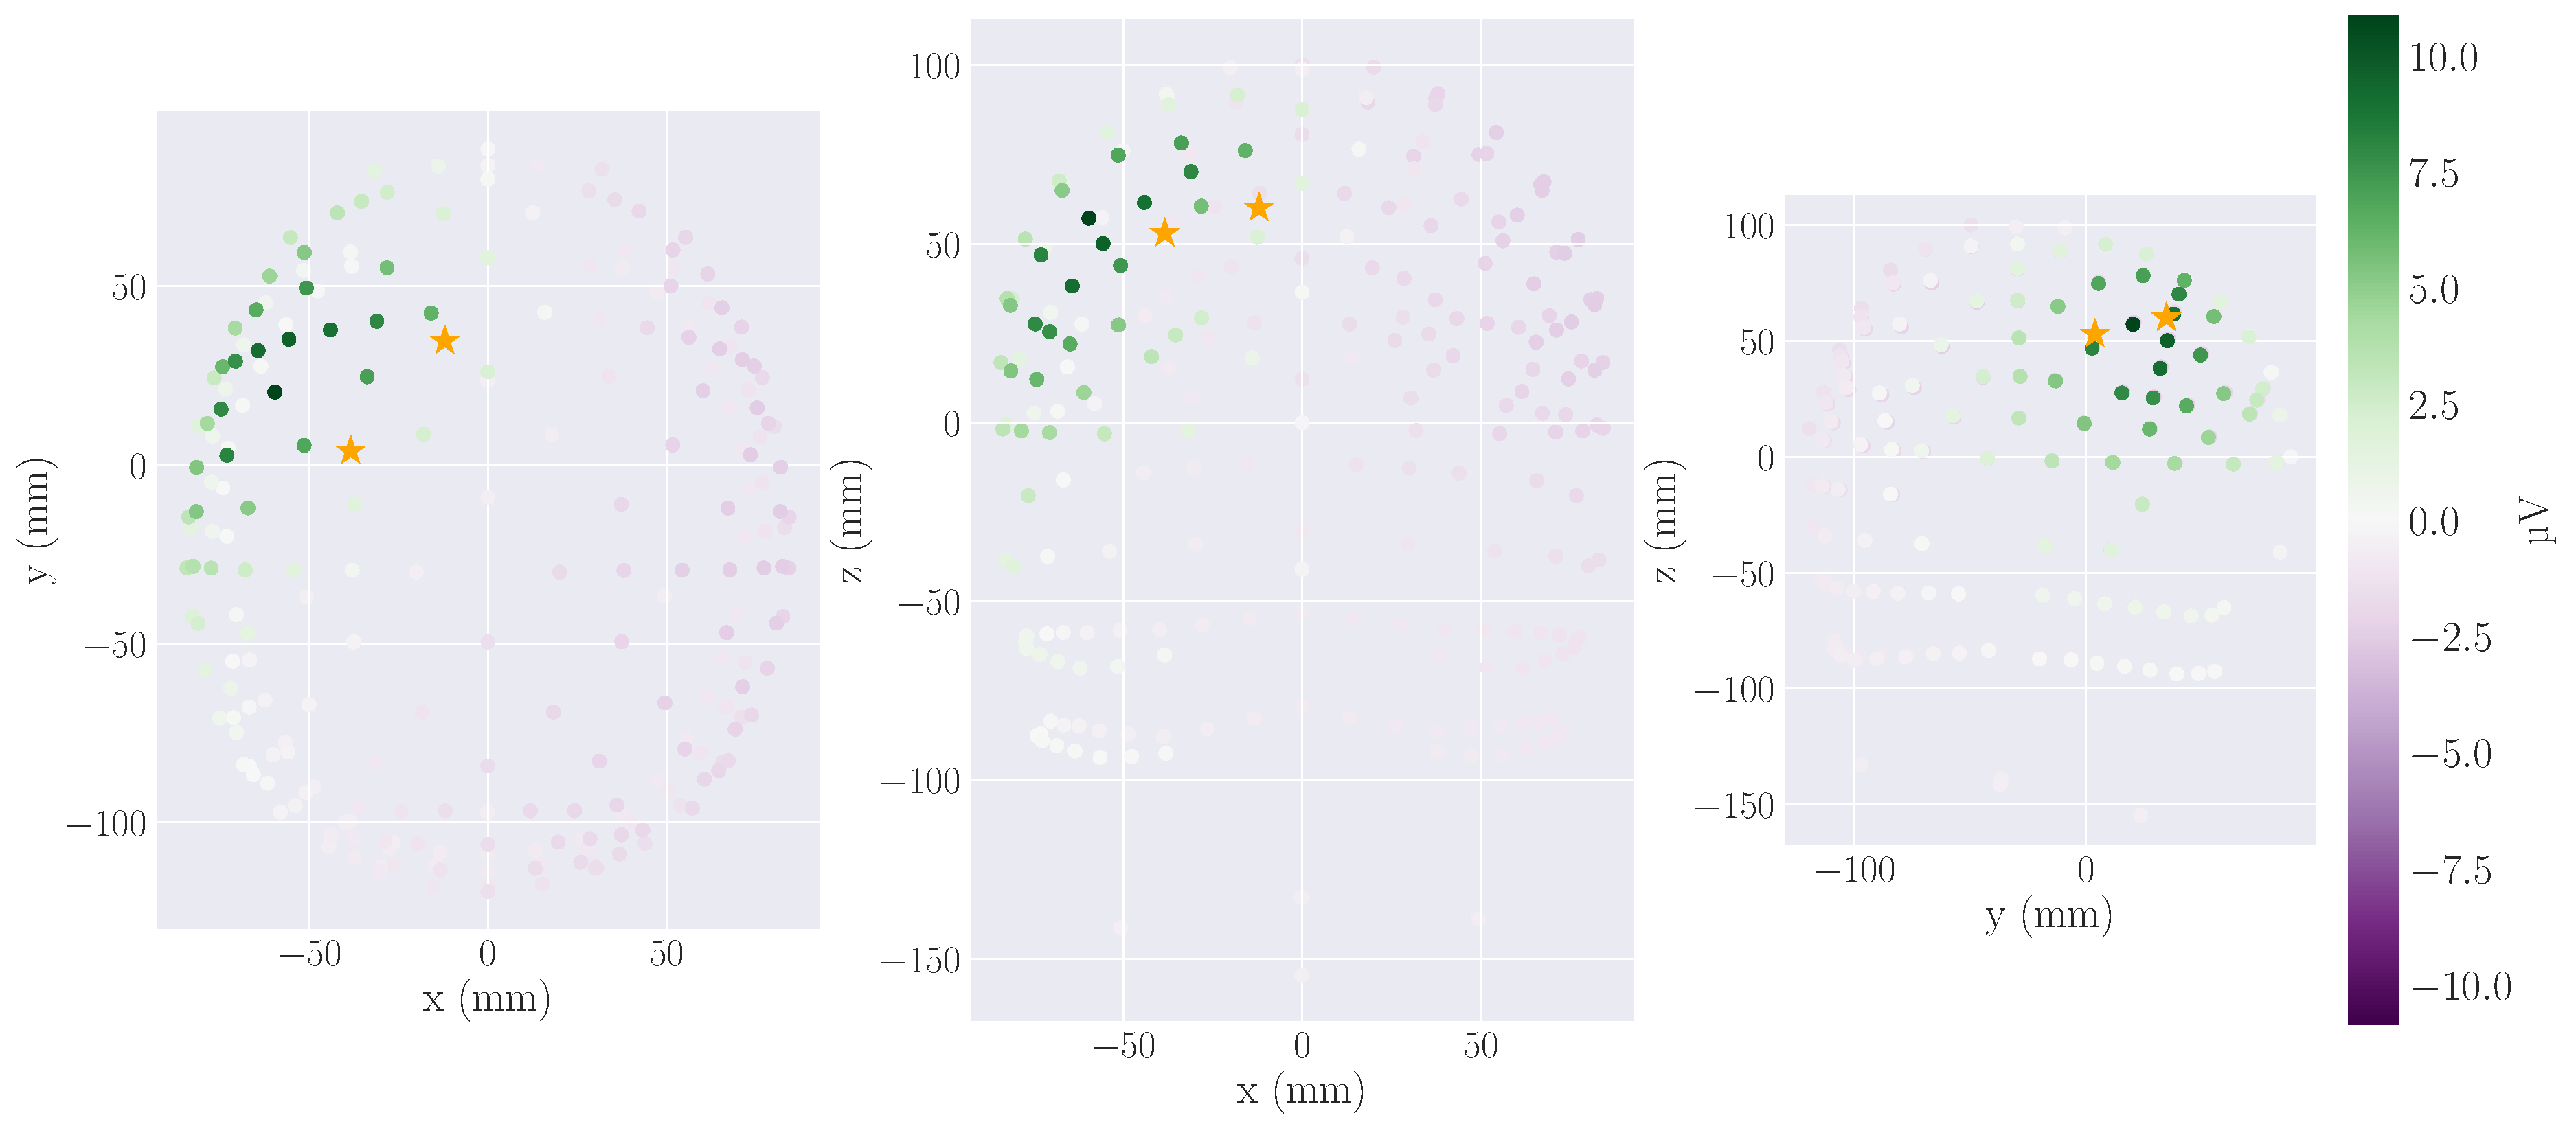
\includegraphics[width=\linewidth]{figures/purple_green/dipoles_w_amplitudes_eeg_field_2_0.pdf}
% 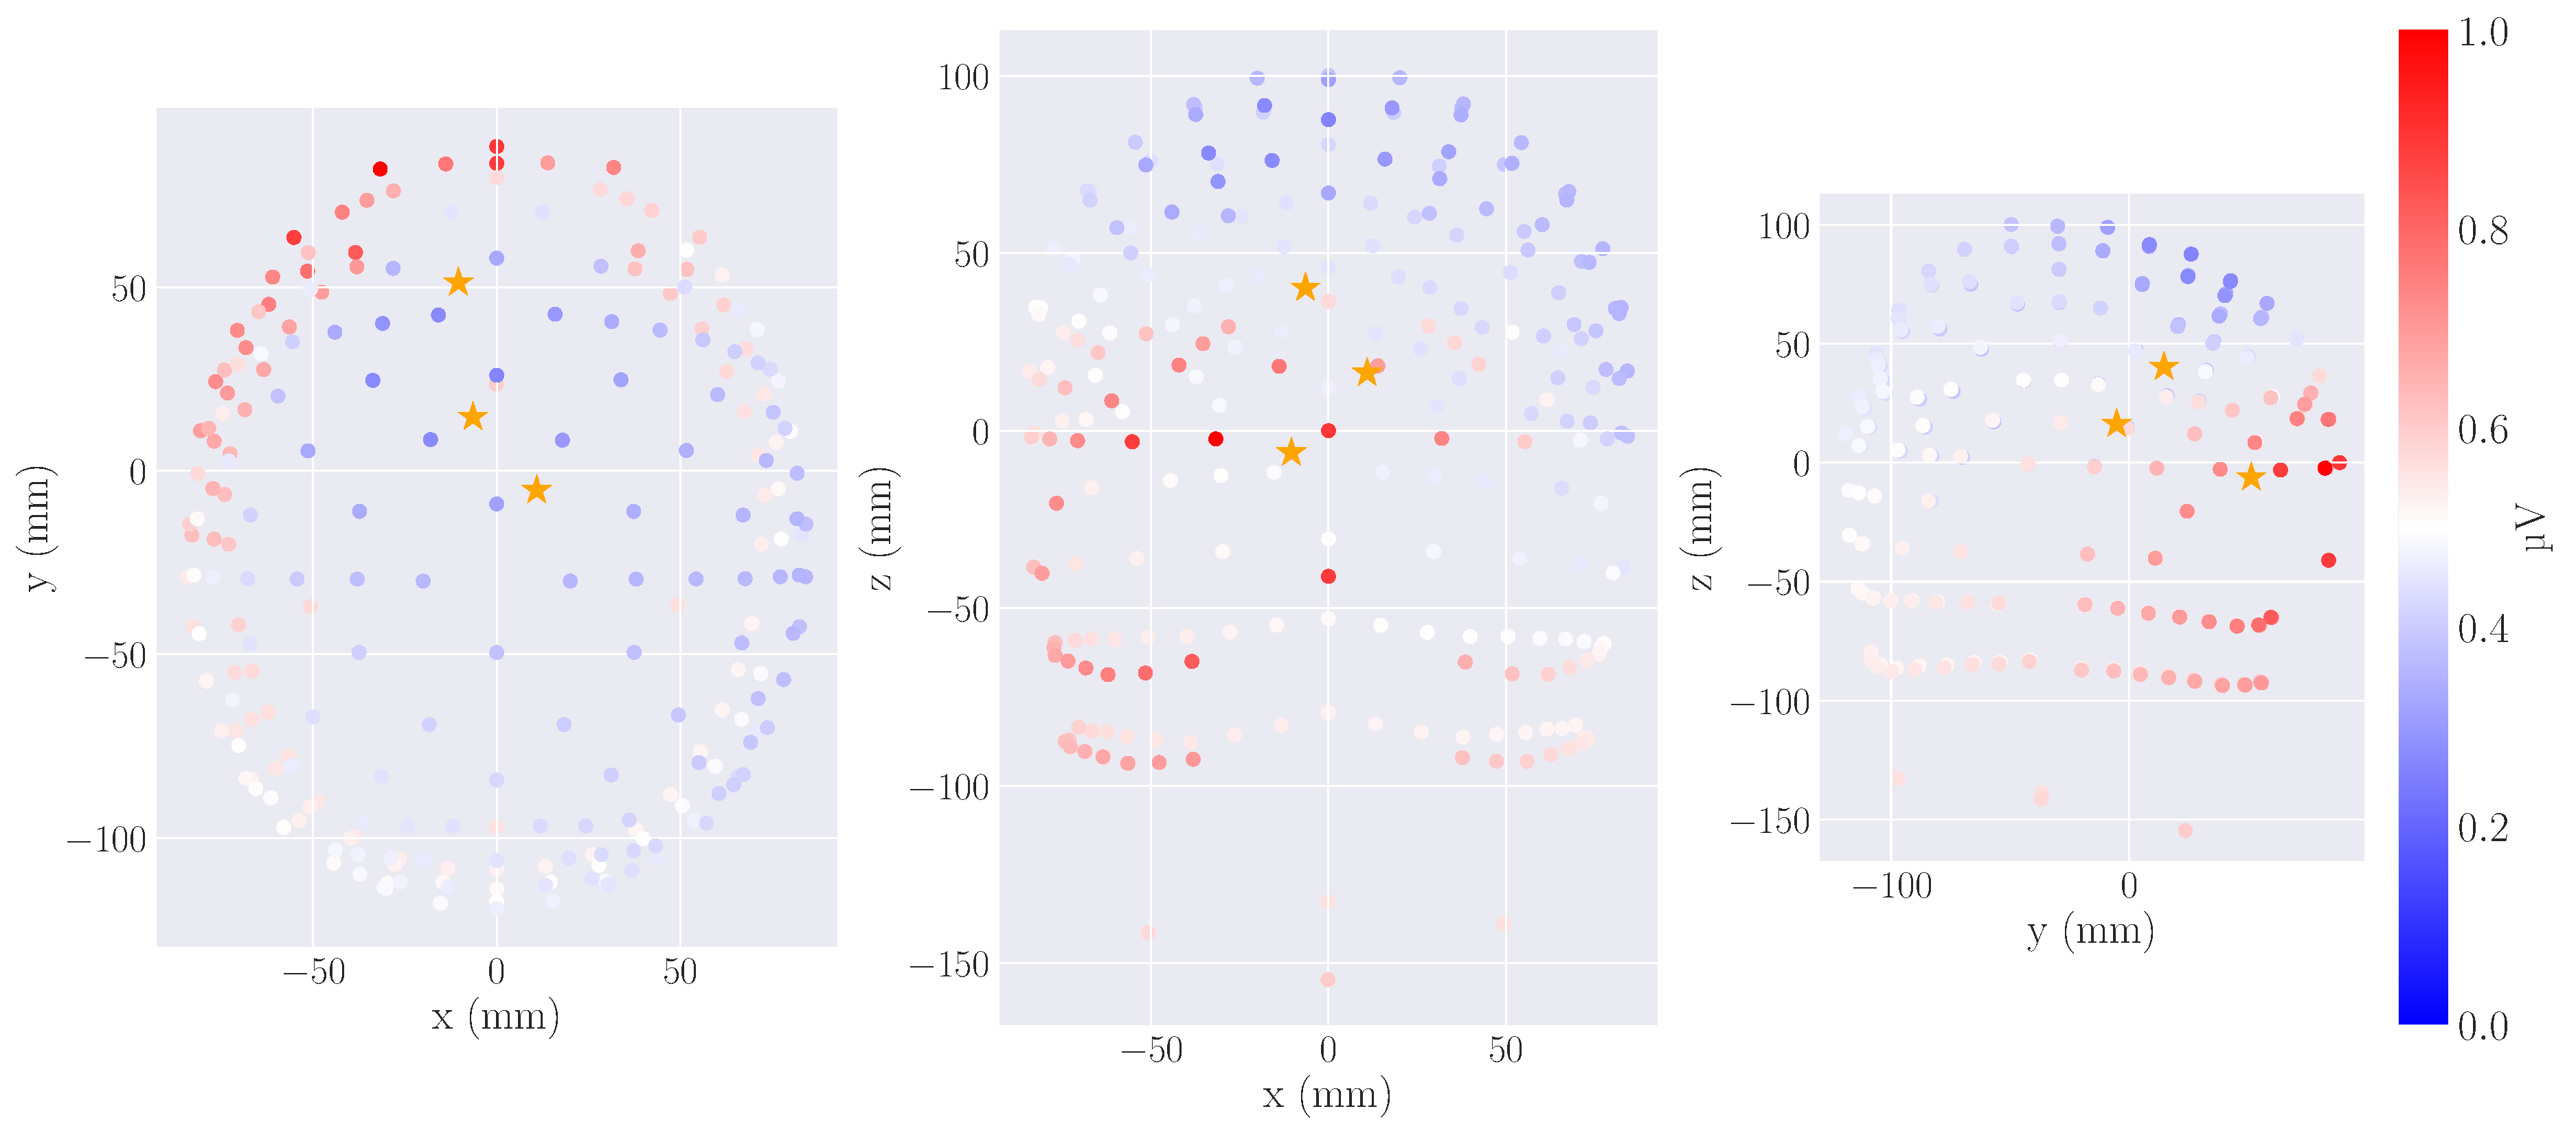
\includegraphics[width=\linewidth]{figures/dipoles_w_amplitudes_eeg_field_3_1.pdf}
\caption{EEG data for a randomly selected sample from the data set containing two dipole sources. These dipoles are positioned at random locations within the cerebral cortex. The EEG measurements are visualized from different perspectives: from above the skull in the $xy$-plane, from the front in the $xz$-plane, and from the side in the $yz$-plane. The EEG electrode locations are represented as filled circles, with the color fill indicating the amplitude of the measured signal at each electrode. The positions of the current dipole moments are marked with yellow stars.}
\label{fig:multiple_dipoles_data}
\end{figure}

\FloatBarrier

In this more complex problem, the total number of target values has increased to six, covering the $x-$, $y-$, and $z-$coordinates for the location of each dipole. However, the network architecture still maintains its 231 input nodes. The number of hidden layers and nodes, the use of dropout techniques, network weight initialization, choice of activation functions, and other hyperparameters largely mirrors those employed in the single current dipole problem for both networks. However, one notable adjustment has been made to the weight decay value in the FFNN network. This hyperparameter has been fine-tuned to 0.1, as this change resulted in a slightly enhanced performance compared to the previous setting of 0.5 used in the single dipole problem.

\section{Customized cost function}
Our new objective is to build a model capable of accurately predicting the positions of not just \emph{one} but \emph{two} dipoles contributing to an EEG signal. To achieve this, we extend the mean Euclidean distance (MED) cost function used in the previous problem for localizing single dipoles. The extended MED function is represented as follows:
\begin{equation}
\begin{aligned}
    \text{MED}(\mathbf{r_1}, \mathbf{r_2}) = \frac{1}{\rednote{2}n}\sum_{i=1}^{n}\sum_{j=1}^{m} \sqrt{(x_{i,j} - \tilde{x_{i,j}})^2 + (y_{i,j} - \tilde{y_{i,j}})^2 + (z_{i,j} - \tilde{z_{1,i}})^2}.
\end{aligned}
\label{eq:MED_multiple_dipoles}
\end{equation}
In this equation, the variable $n$ denotes the total number of samples, while $m$ represents the number of dipoles under consideration. However, given that our task involves localizing two distinct dipoles, our target vector encompasses two sets of coordinates representing the positions of these dipoles that we aim to predict. Consequently, the neural network also produces an output vector containing two sets of coordinates. Conventional cost functions, including the MED utilized for the single dipole problem, typically assume a one-to-one mapping between the first set of coordinates in the target and the first set of coordinates in the network's output. This rigid mapping assumes the order of these elements without flexibility. Such an approach may overlook the possibility that the other permutation of coordinates may be the correct mapping.

The primary task of our neural network is to discern patterns and learn from the input EEG data. Without explicit instructions, the network cannot inherently determine the correct order in which to arrange the coordinates of the two dipoles in its output vector (i.e., which should come first or second). Neglecting this potential permutation ambiguity could lead to suboptimal mappings, subsequently affecting the weight updates during loss calculation.

To overcome this challenge, we instruct the customized cost function to systematically explore all possible permutations of target and output vectors. This approach ensures that all valid combinations are considered, allowing us to determine which permutation yields the minimum loss. During each epoch, the network calculates the loss (Equation \ref{eq:MED_multiple_dipoles}) for each permutation, ultimately selecting the permutation that results in the smallest loss. This process is repeated for every epoch, facilitating more precise weight updates and adaptation. To validate the intended functionality of the customized cost function, we have developed several unit tests, which can be found on our \rednote{GitHub} repository. This customized cost function is designed to accommodate an arbitrary number of dipoles.


\section{Performance Evaluation using the FCNN}
\rednote{Time. 27 sec, 6 hours}
In Figure \ref{fig:two_dipole_result_FFNN}, we display the training and validation mean Euclidean distance loss as a function of training epochs. Our network underwent 800 training epochs, with each lasting approximately 27 seconds. It is noteworthy that the validation loss ceased to improve significantly between 200 and 300 epochs, suggesting that training could have been terminated before reaching 800 epochs. The training loss also plateaued after 400 epochs, demonstrating no signs of overfitting. Both training and validation losses exhibited considerable fluctuations until reaching epoch 190. At epoch 191, the learning rate was reduced to 0.0002, resulting in a significant decline of the validation loss and eliminating further fluctuations. The validation loss eventually stabilized at a value of 18.71 mm by epoch 800, starting from an initial loss of 105.90 mm. We emphasize that this loss represents the mean Euclidean distance for two dipoles. If we want to calculate the mean Euclidean distance for a single dipole alone, we would need to divide this measure by 2, as we will be doing in the results presented from here.


% Figure \ref{fig:NN_multiple_dipoles_architecture} illustrates the updated network architecture.
%Since we constrained each dipole within a sample to have the same amplitude, it is not necessary to have separate output values for the amplitudes of each dipole. Nevertheless, we modified the architecture of the network, considering the possibility of outputting amplitude target values with varying values for each dipole.

% \begin{figure}[!htb]
%   \centering
%   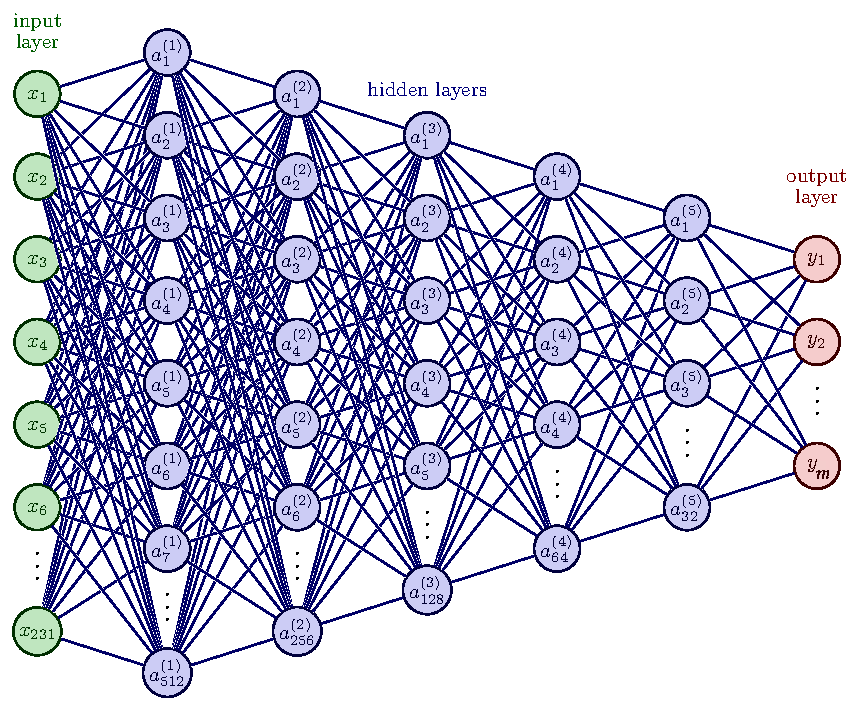
\includegraphics[width=\linewidth]{figures/NN_multiple_outputs.pdf}
%   \caption{Architecture of the multiple dipoles network.}
%   \label{fig:NN_multiple_dipoles_architecture}
% \end{figure}

\begin{figure}[!htb]
    \centering
    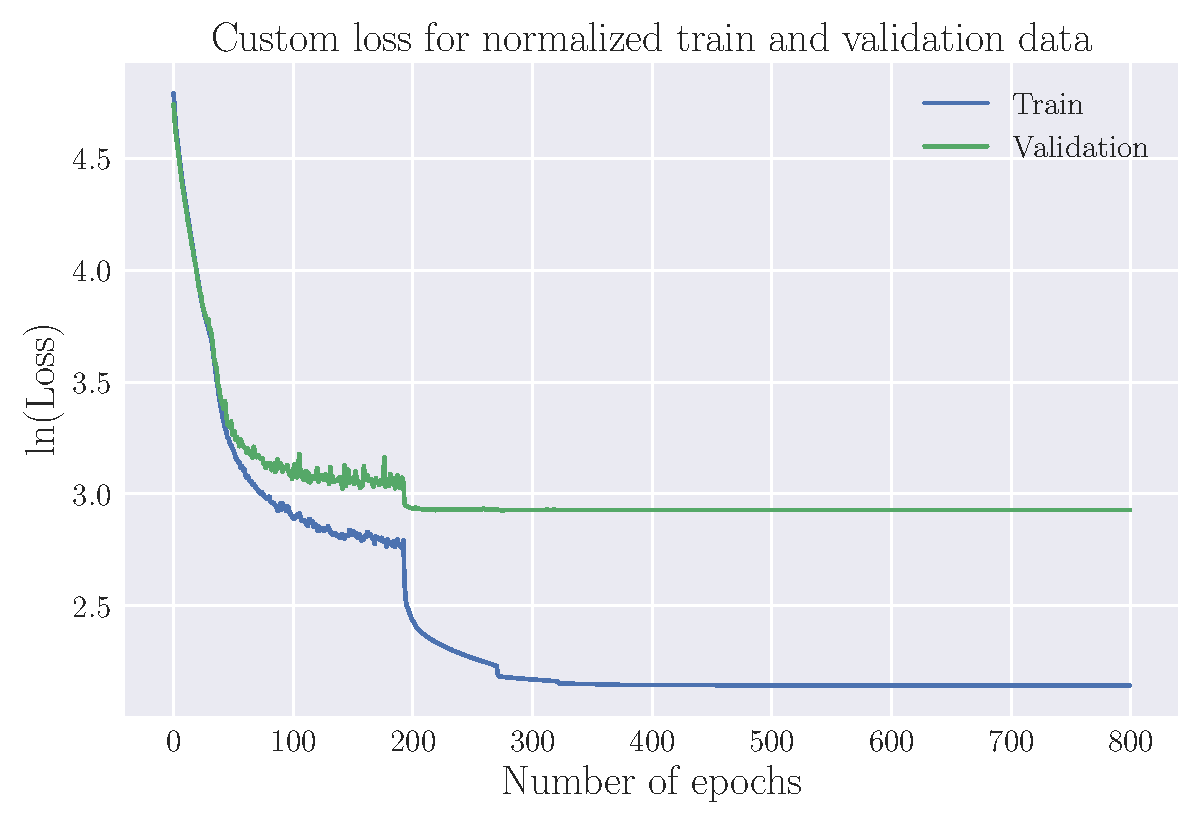
\includegraphics[width=\linewidth]{figures/NN_two_dipole/Custom_Loss_simple_last_run_old_std_2_dipoles_32_0.001_0.35_0.1_0_800_(0).pdf}
    \caption{Training- and validation loss for the FFNN, predicting two current dipole sources, as function of epochs.}
    \label{fig:two_dipole_result_FFNN}
\end{figure}

\FloatBarrier

\rednote{Bør jeg skrive med 3 desimaler eller runde av slik som jeg har gjort her?}
The mean Euclidean distance between predicted and target dipole locations within the EEG test data originating from two current dipoles is 17.41 mm. This indicates that the average error for a single dipole's position is 8.71 mm. Table \ref{table:MED} provides an evaluation of the model's accuracy concerning the Euclidean distance (ED) (averaged over the two dipoles in each sample) between predicted and target dipole positions within the test data set. The FFNN demonstrates an accuracy of less than 15 mm for 90.85$\%$ of the samples in the test data set. However, as the ED threshold becomes stricter at 10 mm and further at 5 mm, the accuracy decreases to 73.06$\%$ and 19.00$\%$, respectively. To visualize the distribution of localization errors across the data set, Figure \ref{fig:two_dipole_result_hist} presents a histogram of the ED between predicted and target positions for 20,000 test samples. The data is grouped into bins with a width of 3 mm. Each bin represents the number of samples with prediction errors falling within the specified interval. This histogram reveals that the majority of predictions exhibit errors smaller than 15 mm. Nonetheless, approximately 10$\%$ of the predictions fall outside this threshold.

\begin{table}[]
  \centering
\begin{tabular}{|ccc|}
\hline
\rowcolor[HTML]{CBCEFB}
\multicolumn{3}{|c|}{\cellcolor[HTML]{CBCEFB}\textbf{Euclidian Distance for Test Samples}}                                                             \\ \hline
\rowcolor[HTML]{EFEFEF}
\multicolumn{1}{|c|}{\cellcolor[HTML]{EFEFEF}ED \textless 5 mm} & \multicolumn{1}{c|}{\cellcolor[HTML]{EFEFEF}ED \textless 10 mm} & ED \textless 15 mm \\ \hline
\rowcolor[HTML]{FFFFFF}
\multicolumn{1}{|c|}{\cellcolor[HTML]{FFFFFF}18.995 $\%$}       & \multicolumn{1}{c|}{\cellcolor[HTML]{FFFFFF}73.055 $\%$}        & 90.850 $\%$        \\ \hline
\end{tabular}
\caption{\textbf{ED between targets and predictions of test samples; Predicting Two Dipole Locations with the FFNN} \newline
Performance of the FFNN on the test data set comprising 20,000 samples, presented as the percentage of samples falling within ED thresholds of 5 mm, 10 mm and 15 mm respectively.}
\label{table:MED}
\end{table}

\begin{figure}[!htb]
    \centering
    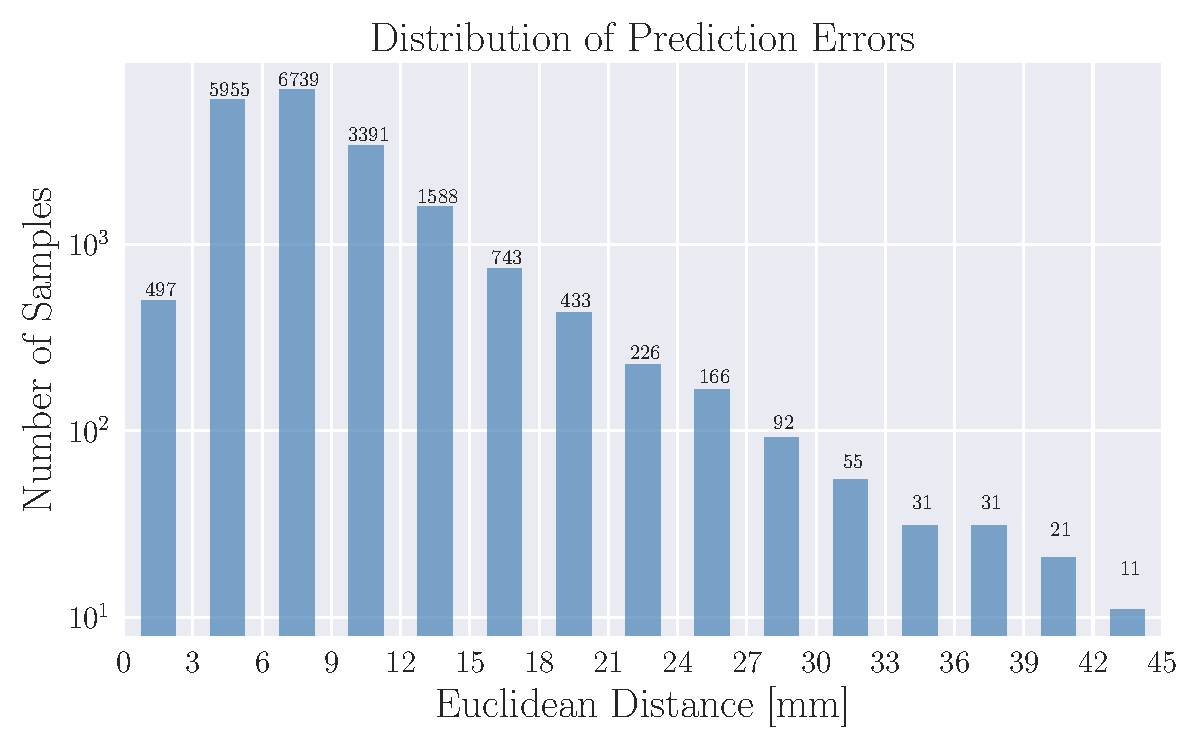
\includegraphics[width=\linewidth]{figures/NN_two_dipole/new_histogram_2_dipoles_position_amplitude.pdf}
    \caption{Histrogram illustrating the Euclidean Distance for predicted dipole locations, organized into bins of width 3 mm. The ED thresholds are organized into bins of width 3 mm. Each bin holds the number of samples with prediction errors that falls within the given interval. }
    \label{fig:two_dipole_result_hist}
\end{figure}

Table \ref{table:error_multiple_dipoles} offers further evaluation of the model's performance using various error metrics. The MAE for the $x$-, $y$-, and $z$-coordinates of the dipole positions are all below 5 mm, indicating precise predictions in these dimensions. However, the MSE values, ranging from 36.98 mm$^2$ to 40.83 mm$^2$, are considerable higher than those observed in the single dipole case, signifying increased error spread in this more complex scenario. RMSE averages at 6.243 mm, further confirming the model's higher error spred.

Once again, we observe slightly higher errors in all metrics when predicting the $z$-coordinate of the dipole source, suggesting that accurately predicting this spatial coordinate remains a somewhat greater challenge for the FFNN in this multi-dipole scenario.

\begin{table}[!htb]
  \centering
\begin{tabular}{l|cccc|}
\cline{2-5}
\rowcolor[HTML]{CBCEFB}
\cellcolor[HTML]{FFFFFF}                           & \multicolumn{4}{c|}{\cellcolor[HTML]{CBCEFB}{\color[HTML]{000000} \textbf{Error Metrics for Target Values}}}                                                                                                                                                                                                                                                                                                                                                     \\ \cline{2-5}
\rowcolor[HTML]{EFEFEF}
\cellcolor[HTML]{FFFFFF}\textbf{}                  & \multicolumn{1}{l|}{\cellcolor[HTML]{EFEFEF}\begin{tabular}[c]{@{}l@{}}x-coordinate\\ {[}mm{]}\end{tabular}} & \multicolumn{1}{l|}{\cellcolor[HTML]{EFEFEF}\begin{tabular}[c]{@{}l@{}}y-coordinate \\ {[}mm{]}\end{tabular}} & \multicolumn{1}{l|}{\cellcolor[HTML]{EFEFEF}\begin{tabular}[c]{@{}l@{}}z-coordinate \\ {[}mm{]}\end{tabular}} & \multicolumn{1}{l|}{\cellcolor[HTML]{EFEFEF}\begin{tabular}[c]{@{}l@{}}Position \\ Error {[}mm{]}\end{tabular}} \\ \hline
\multicolumn{1}{|l|}{\cellcolor[HTML]{EFEFEF}MAE}  & \multicolumn{1}{c|}{4.156}                                                                                  & \multicolumn{1}{c|}{4.379}                                                                                   & \multicolumn{1}{c|}{4.485}                                                                                   & 4.340                                                                                                              \\ \hline
\multicolumn{1}{|l|}{\cellcolor[HTML]{EFEFEF}MSE}  & \multicolumn{1}{c|}{36.977}                                                                                  & \multicolumn{1}{c|}{39.122}                                                                                   & \multicolumn{1}{c|}{40.834}                                                                                   & 38.978                                                                                                              \\ \hline
\multicolumn{1}{|l|}{\cellcolor[HTML]{EFEFEF}RMSE} & \multicolumn{1}{c|}{6.081}                                                                                  & \multicolumn{1}{c|}{6.255}                                                                                   & \multicolumn{1}{c|}{6.390}                                                                                   & 6.243                                                                                                              \\ \hline
\end{tabular}
\caption{\textbf{FFNN: Evaluation of the network's performance utializing different Error Metrics.} \newline
FFNN performance on test data set consisting of 20,000 samples. The errors are measured using Mean Squared Error (MSE), Mean Absolute Error (MAE), and Root Mean Squared Error (RMSE).}
\label{table:error_multiple_dipoles}
\end{table}

For illustrative purposes, we examine a specific prediction from our model. Consider a sample containing two dipoles located at $\tilde{\mathbf{r_1}}$ = (52.53, -16.25, 8.60) and $\tilde{\mathbf{r_2}}$ = (-63.48, -45.06, 22.67) in units of mm. Our model predicts the positions $\mathbf{r_1}$ = (55.95, -17.07, 13.43) and $\mathbf{r_2}$ = (-64.09, -48.73, 19.89) in units of mm, respectively. This results in an Euclidean distance of approximately 5.98 mm between $\tilde{\mathbf{r_1}}$ and $r_1$, and approximately 4.65 mm between $\tilde{\mathbf{r_2}}$ and $\mathbf{r_2}$. Although this prediction exhibits a slightly larger localization error compared to the single-dipole scenario, it still falls below the 1 cm threshold we aim for.
It is however important to note that this example represents one of the better-performing predictions, as only 19$\%$ of the test data set's predictions falls below a precision of 5 mm. In Figure \ref{fig:two_dipole_result}, we visualize the predicted positions ($\mathbf{r_1}$ and $\mathbf{r_2}$) of the dipoles alongside the target positions ($\mathbf{\tilde{r_1}}$ and $\mathbf{\tilde{r_2}}$).

\begin{figure}[!htb]
  \hspace*{-4.5cm}
    \centering
    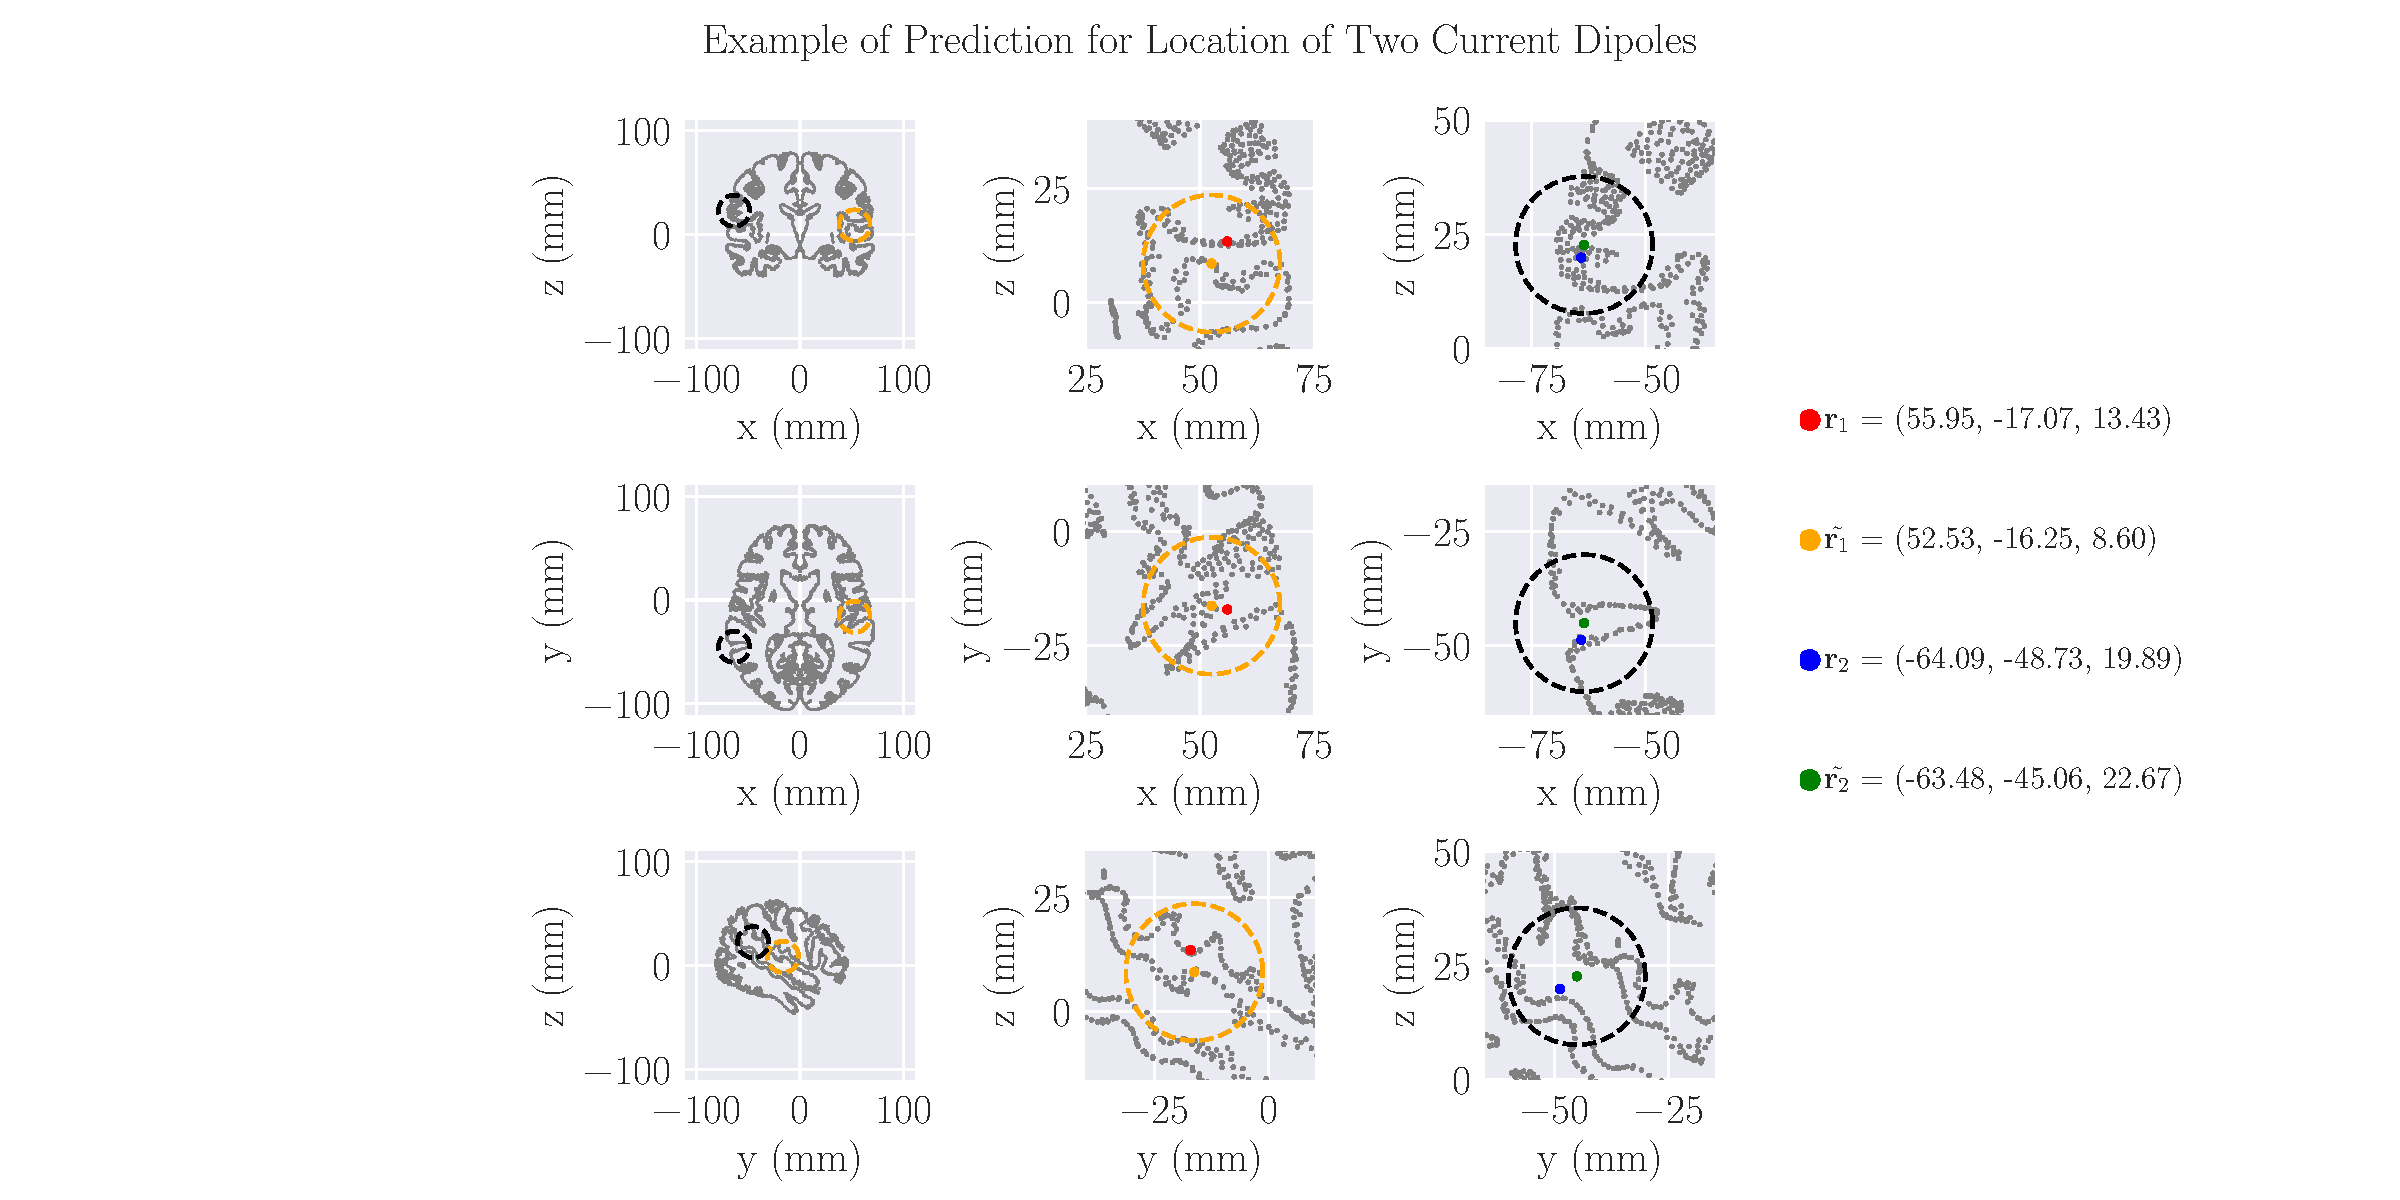
\includegraphics[width=20cm]{figures/NN_two_dipole/two_dipoles_prediction.pdf}
    \caption{Depiction of prediction and true value of the locations of two current dipoles within a sample from the test data set.}
    \label{fig:two_dipole_result}
\end{figure}

\FloatBarrier


\section{Performance Evaluation using the CNN}
\rednote{}
We proceed to assess the performance of our Convolutional Neural Network in the task of predicting the positions of two current dipoles within the NY cortex. In Figure \ref{fig:two_dipole_result_CNN}, we present the training and validation mean Euclidean distance loss as function of training epochs. The CNN underwent a training process, comprising 800 epochs, with each epoch requiring approximately 40 seconds to complete. This training duration represents a slight increase compared to the FFNN. Analogous to our observations with the FFNN model, we noted that the validation loss stabilized around epoch 300, suggesting that an earlier termination of training could have been considered. The training loss, much like the FFNN, reached a plateau after 400 epochs, indicating the absence of overfitting. The learning rate scheduling, mitigate fluctuations in the validation loss, where the learning rate was decreased to 0.0002 at epoch 250, leading to a decline in the validation loss and eventual stabilization at a value of 19.65 mm by epoch 800. Notably, this final validation loss is somewhat higher than that achieved by the FFNN.


\begin{figure}[!htb]
    \centering
    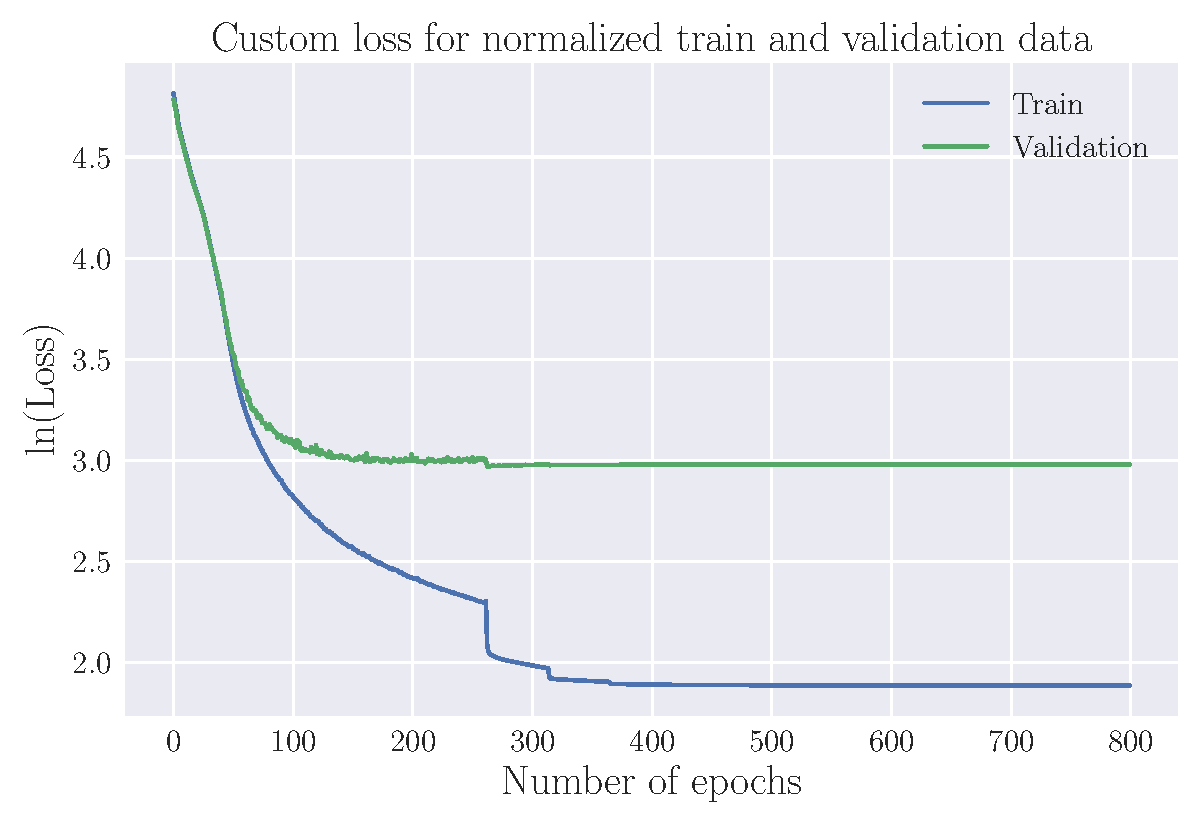
\includegraphics[width=\linewidth]{figures/CNN/Custom_Loss_simple_last_run_old_std_2_dipoles_32_0.001_0.35_0.5_0_800_(0).pdf}
    \caption{Training- and validation loss for the CNN, predicting two current dipole sources, as function of epochs.}
    \label{fig:two_dipole_result_CNN}
\end{figure}

\FloatBarrier

Table \ref{table:MED} provides an evaluation of the CNN's accuracy, expressed in terms of the Euclidean distance between predicted and target dipole positions for the test data set. The CNN demonstrates an accuracy smaller than 15 mm for 78.87$\%$ of the test samples. However, as the ED threshold is progressively tightened to 10 mm and subsequently to 5 mm, the accuracy diminishes to 50.46$\%$ and 7.55$\%$, respectively. To provide a visual representation of the distribution of localization errors, Figure \ref{fig:two_dipole_result_hist} showcases a histogram of the ED between predicted and target positions for 20,000 test samples, organized into bins of width 3 mm. As lined out in the previous result section for the FFNN each bin represents the number of samples with prediction errors falling within the specified interval with range 3 mm. However, in contrast to the FFNN model, this histogram reveals that while most predictions exhibit errors smaller than 15 mm, a significant proportion experiences higher errors, with approximately 20$\%$ falling beyond this threshold, which is a double from what we saw with the FFNN.

\begin{table}[]
  \centering
\begin{tabular}{|ccc|}
\hline
\rowcolor[HTML]{CBCEFB}
\multicolumn{3}{|c|}{\cellcolor[HTML]{CBCEFB}\textbf{Euclidian Distance for Test Samples}}                                                             \\ \hline
\rowcolor[HTML]{EFEFEF}
\multicolumn{1}{|c|}{\cellcolor[HTML]{EFEFEF}ED \textless 5 mm} & \multicolumn{1}{c|}{\cellcolor[HTML]{EFEFEF}ED \textless 10 mm} & ED \textless 15 mm \\ \hline
\rowcolor[HTML]{FFFFFF}
\multicolumn{1}{|c|}{\cellcolor[HTML]{FFFFFF}7.545 $\%$}       & \multicolumn{1}{c|}{\cellcolor[HTML]{FFFFFF}50.460 $\%$}        & 78.870 $\%$        \\ \hline
\end{tabular}
\caption{\textbf{ED between targets and predictions of test samples; Predicting Two Dipole Locations with CNN} \newline
Performance of the network on the test data set comprising 20,000 samples, presented as the percentage of samples falling within ED thresholds of 5 mm, 10 mm and 15 mm respectively.}
\label{table:MED}
\end{table}

\begin{figure}[!htb]
    \centering
    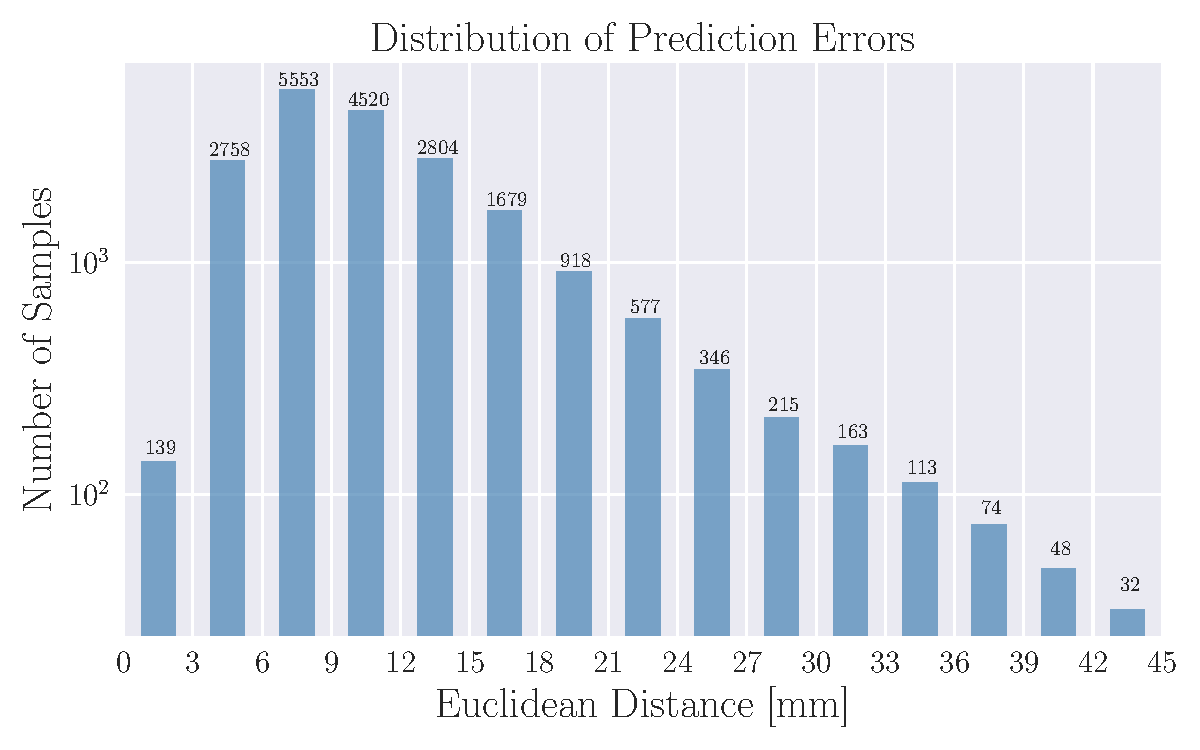
\includegraphics[width=\linewidth]{figures/CNN/new_histogram_2_dipoles_position_simple_cnn.pdf}
    \caption{Histrogram illustrating the Euclidean Distance for predicted dipole locations, organized into bins of width 3 mm.}
    \label{fig:two_dipole_result_hist}
\end{figure}

Table \ref{table:error_multiple_dipoles} provides a comprehensive evaluation of the CNN's performance, employing various error metrics. The MAE for the $x$, $y$, and $z$-coordinates of the dipole positions averages at 5.40 mm, indicating accurate localization predictions in these spatial dimensions. However, the MSE values, ranging from 63.53 mm$^2$ to 79.95 mm$^2$, are higher than the corresponding values observed in the FFNN model, suggesting a broader dispersion of errors. The RMSE averages at 8.397 mm. Consistent with the single-dipole problem and the FFNN's performance in this multi-dipole problem, we observe somewhat higher errors across all metrics when predicting the $z$-coordinate of the dipole sources. This suggests that accurate $z$-coordinate prediction remains the most challenging target. However, it is important to note that the increase in errors is modest and should not be considered significant without further investigation.

\begin{table}[!htb]
  \centering
\begin{tabular}{l|cccc|}
\cline{2-5}
\rowcolor[HTML]{CBCEFB}
\cellcolor[HTML]{FFFFFF}                           & \multicolumn{4}{c|}{\cellcolor[HTML]{CBCEFB}{\color[HTML]{000000} \textbf{Error Metrics for Target Values}}}                                                                                                                                                                                                                                                                                                                                                     \\ \cline{2-5}
\rowcolor[HTML]{EFEFEF}
\cellcolor[HTML]{FFFFFF}\textbf{}                  & \multicolumn{1}{l|}{\cellcolor[HTML]{EFEFEF}\begin{tabular}[c]{@{}l@{}}x-coordinate\\ {[}mm{]}\end{tabular}} & \multicolumn{1}{l|}{\cellcolor[HTML]{EFEFEF}\begin{tabular}[c]{@{}l@{}}y-coordinate \\ {[}mm{]}\end{tabular}} & \multicolumn{1}{l|}{\cellcolor[HTML]{EFEFEF}\begin{tabular}[c]{@{}l@{}}z-coordinate \\ {[}mm{]}\end{tabular}} & \multicolumn{1}{l|}{\cellcolor[HTML]{EFEFEF}\begin{tabular}[c]{@{}l@{}}Position \\ Error {[}mm{]}\end{tabular}} \\ \hline
\multicolumn{1}{|l|}{\cellcolor[HTML]{EFEFEF}MAE}  & \multicolumn{1}{c|}{5.395}                                                                                  & \multicolumn{1}{c|}{5.534}                                                                                   & \multicolumn{1}{c|}{6.265}                                                                                   & 5.731                                                                                                              \\ \hline
\multicolumn{1}{|l|}{\cellcolor[HTML]{EFEFEF}MSE}  & \multicolumn{1}{c|}{63.533}                                                                                  & \multicolumn{1}{c|}{64.433}                                                                                   & \multicolumn{1}{c|}{79.952}                                                                                   & 69.306                                                                                                             \\ \hline
\multicolumn{1}{|l|}{\cellcolor[HTML]{EFEFEF}RMSE} & \multicolumn{1}{c|}{7.971}                                                                                  & \multicolumn{1}{c|}{8.027}                                                                                   & \multicolumn{1}{c|}{8.942}                                                                                   & 8.325                                                                                                              \\ \hline
\end{tabular}
\caption{\textbf{CNN: Evaluation of the network's performance utializing different Error Metrics.} \newline
CNN performance on test data set consisting of 20,000 samples. The errors are measured using Mean Squared Error (MSE), Mean Absolute Error (MAE), and Root Mean Squared Error (RMSE).}
\label{table:error_multiple_dipoles}
\end{table}

% For illustrative purposes, we examine a specific prediction from our model. Consider a sample containing two dipoles located at
% $\tilde{r_1} = [52.53 , \text{mm}, -16.25 , \text{mm}, 8.60 , \text{mm}]$ and
% $\tilde{r_2} = [-63.48 , \text{mm}, -45.06 , \text{mm}, 22.67 , \text{mm}]$.
% Our model predicts the positions $r_1 = [55.95 , \text{mm}, -17.07 , \text{mm}, 13.43 , \text{mm}]$ and $r_2 = [-64.09 , \text{mm}, -48.73 , \text{mm}, 19.89 , \text{mm}]$, respectively. This results in an Euclidean distance of approximately 5.98 mm between $\tilde{r_1}$ and $r_1$, and approximately 4.65 mm between $\tilde{r_2}$ and $r_2$. Although this prediction exhibits a slightly larger localization error compared to the single-dipole scenario, it still falls below the 1 cm threshold we aimed for. It is however important to note that this example represents one of the better-performing predictions, as only 19$\%$ of the test data set's predictions falls below a precision of 5 mm. In Figure \ref{fig:two_dipole_result}, we visualize the predicted positions ($\mathbf{r_1}$ and $\mathbf{r_2}$) of the dipoles alongside the target positions ($\mathbf{\tilde{r_1}}$ and $\mathbf{\tilde{r_2}}$).
%
% \begin{figure}[!htb]
%   \hspace*{-1cm}
%     \centering
%     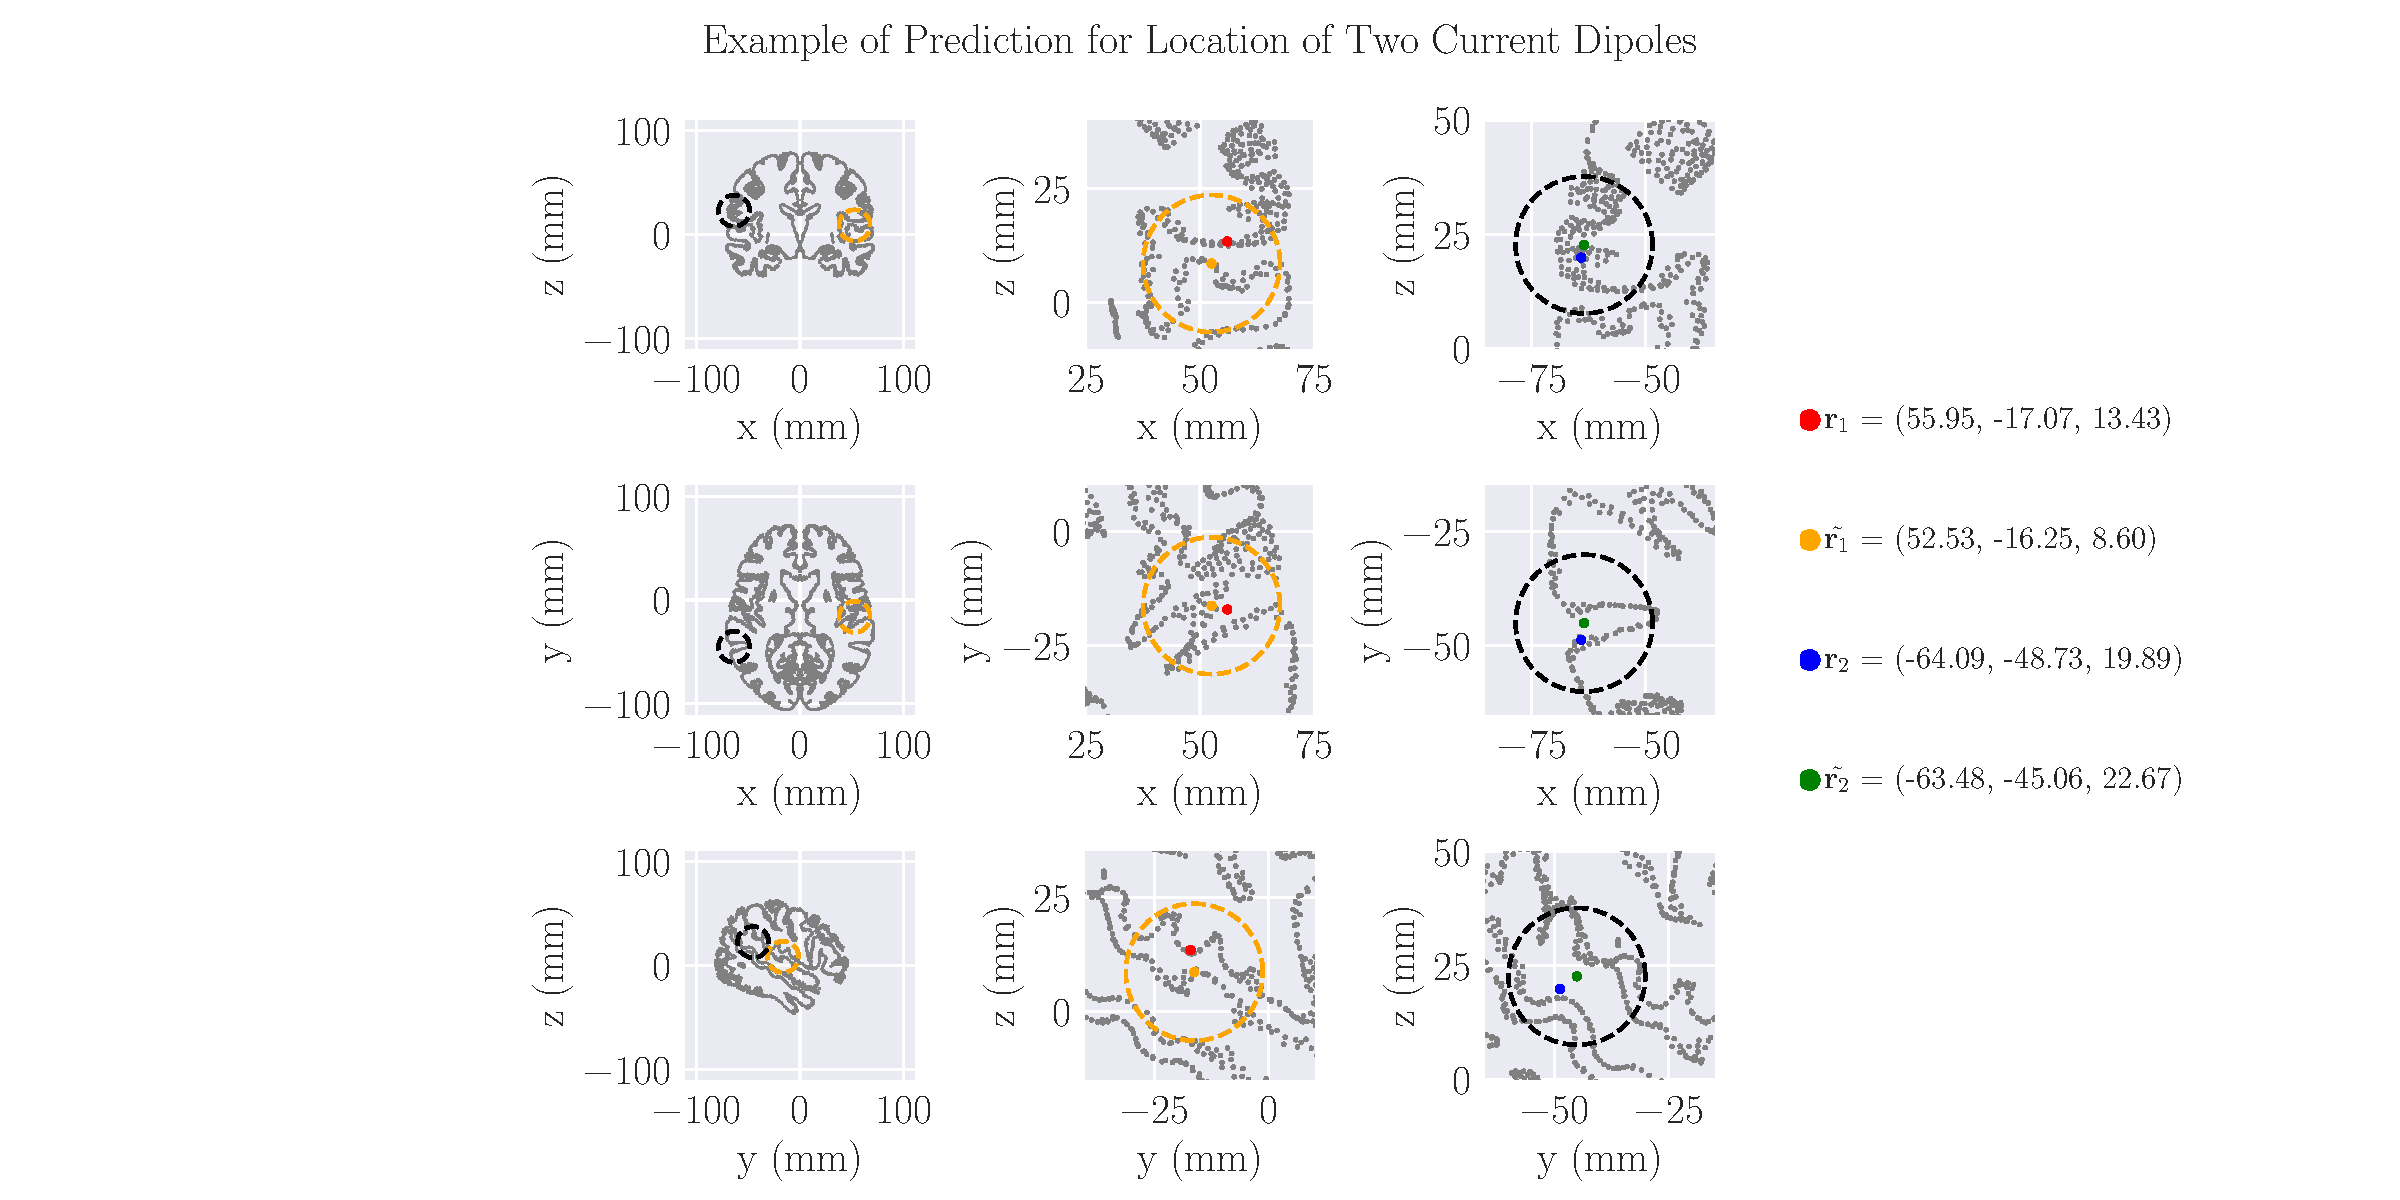
\includegraphics[width=15cm]{figures/NN_two_dipole/two_dipoles_prediction.pdf}
%     \caption{Illustration of prediction and true value of the locations of two current dipoles within a sample from the test data set.}
%     \label{fig:two_dipole_result}
% \end{figure}


\end{document}


